\subsection{Tracking a Single Point}
In order to track a single point, then the equations \ref{eq:tsp_visServoing1} and \ref{eq:tsp_visServoing2} (cite Henriks notes) were implemented.

\begin{eqnarray}
(Z_{image} \cdot Z_{image}^T) y = [du, dv]^T \label{eq:tsp_visServoing1} \\
dq = Z_{image}^T \cdot y \label{eq:tsp_visServoing2}
\end{eqnarray}

Furthermore a time scaling was implemented such that the robot would not move faster than its constraints.
The goal configuration for each frame is furthermore stored such that when a marker is not found in one frame, then the most recent found position is the one the robot moves to.

In order to test the implementation of the algorithm, the marker movement of the three files are stepwise used to update the markers position.
The $dq$ for every step is then computed and used to update the robot.

To find the simulated $(u,v)$ of the marker in the frame of the camera, then the transformation from the camera to the marker ($T_{world}^{camera}$) is found using equation \ref{eq:tsp_TcameraMarker}.

\begin{equation}
T_{world}^{marker} = T_{world}^{camera} \cdot T_{camera}^{marker} \label{eq:tsp_TcameraMarker}
\end{equation}

From $T_{camera}^{marker}$ the positional part is then extracted and used with equation \ref{eq:tsp_u} and \ref{eq:tsp_v} to find $(u,v)$ using the pinhole model.
Where $f$ is the focal length in pixel.

\begin{eqnarray}
u = \frac{f \cdot x}{z} \label{eq:tsp_u} \\
v = \frac{f \cdot y}{z} \label{eq:tsp_v}
\end{eqnarray}


The system was tested on the three marker movements provided and the robot speed is plotted in figure \ref{fig:robotspeed_slow_1p}, \ref{fig:robotspeed_medium_1p} and \ref{fig:robotspeed_fast_1p}.
The tool pose was likewise plotted in figure \ref{fig:toolpose_1p_pos}, \ref{fig:toolpose_slow_1p_rpy}, \ref{fig:toolpose_medium_1p_rpy} and \ref{fig:toolpose_fast_1p_rpy} and the tracking error in image coordinates in figure \ref{fig:trackingerror_slow_1p}, \ref{fig:trackingerror_medium_1p} and \ref{fig:trackingerror_fast_1p}.
The translational part of the toll pose is only plotted along the z- and x-axis since the y values are constant.
The robot joint configurations can be seen in appendix \ref{app:roboticsPlots}.
All figures were plotted with a $\Delta t = 0.05$sec.

% ---------- speeed ----------
\begin{figure}[H]
\centering
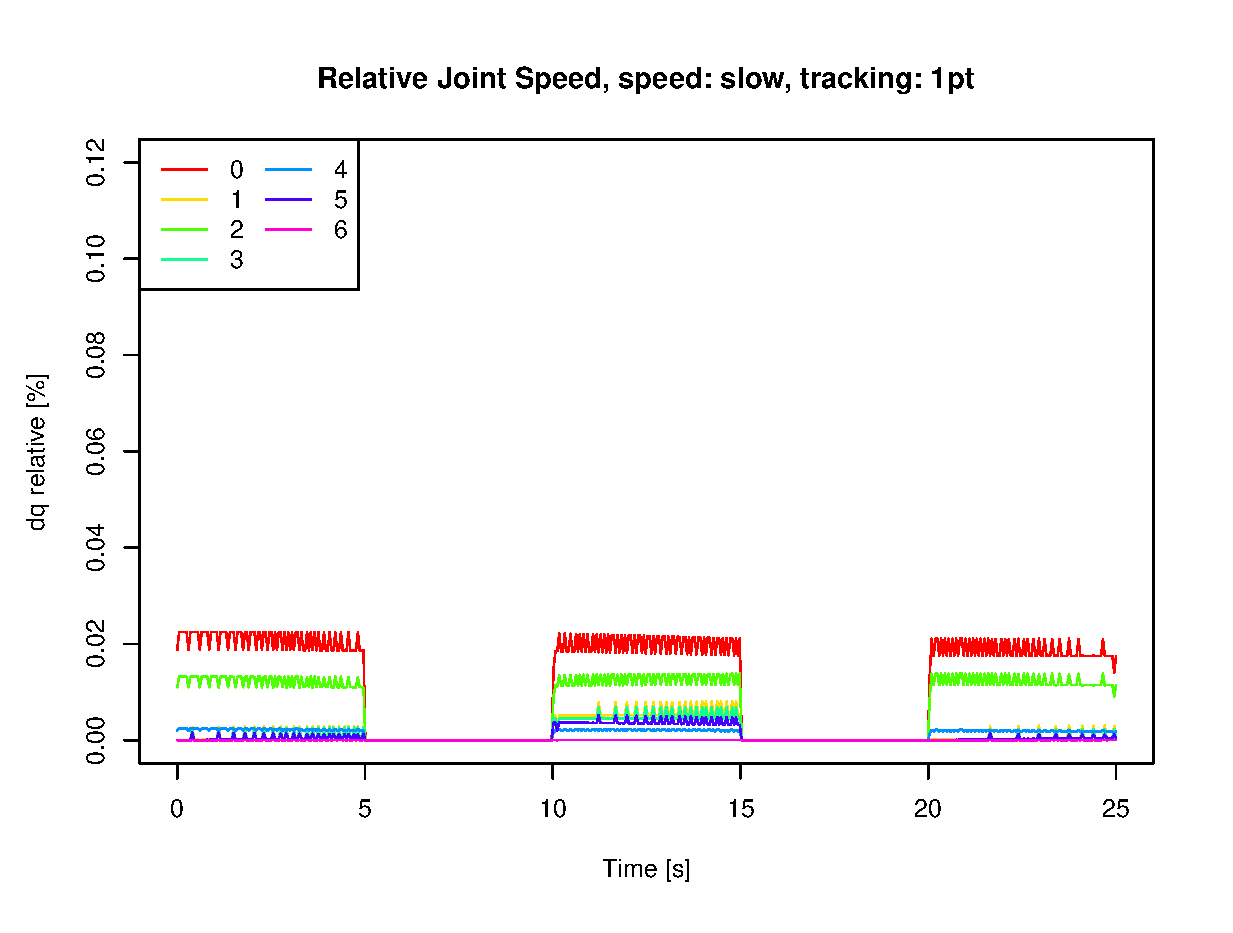
\includegraphics[width= \linewidth]{graphics/robotics/relativeConfVel_slow_1pt}
\caption{Robot speed relative to the velocity limit. 
Tracking one point using slow marker movement.}
\label{fig:robotspeed_slow_1p}
\end{figure}

\begin{figure}[H]
\centering
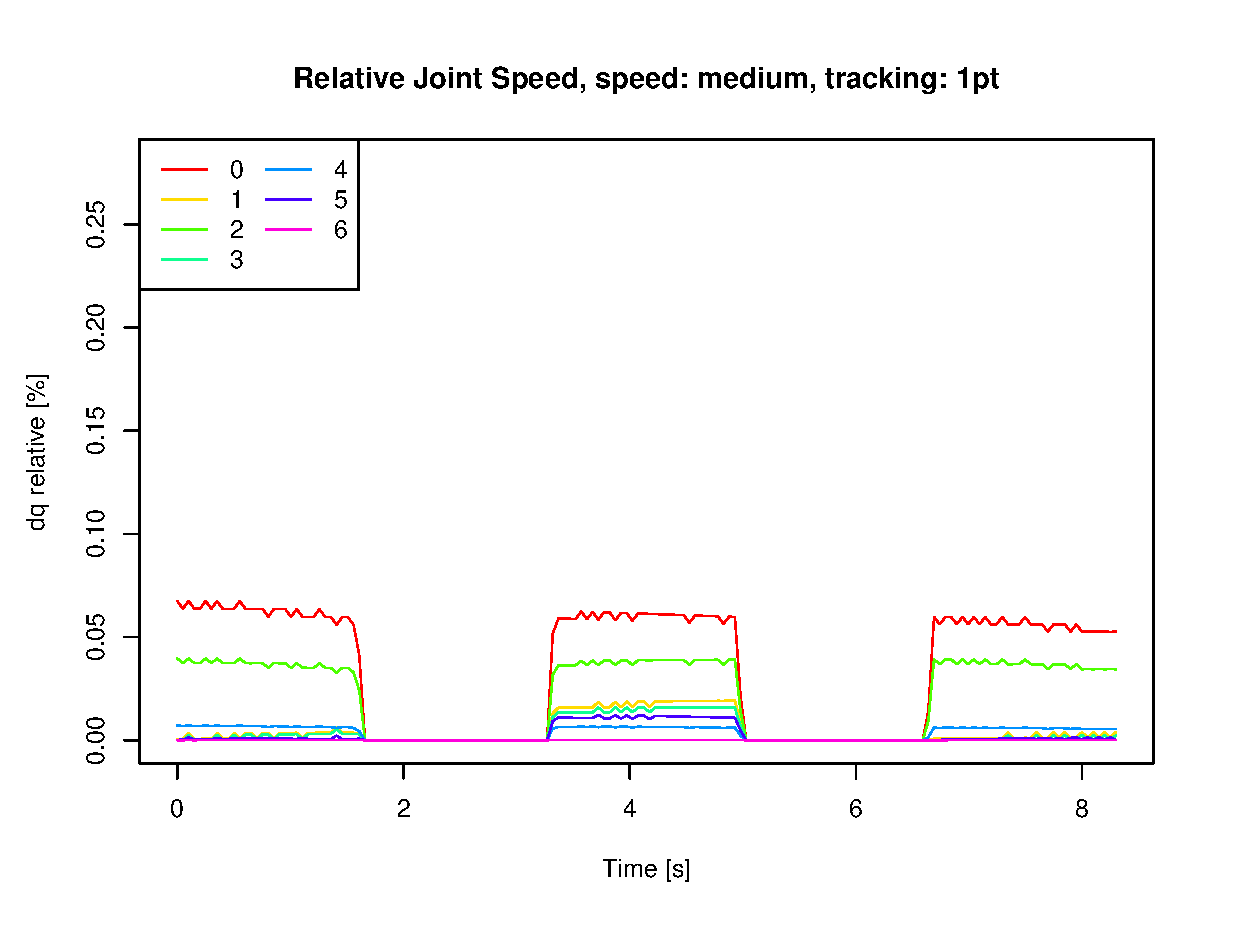
\includegraphics[width= \linewidth]{graphics/robotics/relativeConfVel_medium_1pt}
\caption{Robot speed relative to the velocity limit. 
Tracking one point using medium marker movement.}
\label{fig:robotspeed_medium_1p}
\end{figure}

\begin{figure}[H]
\centering
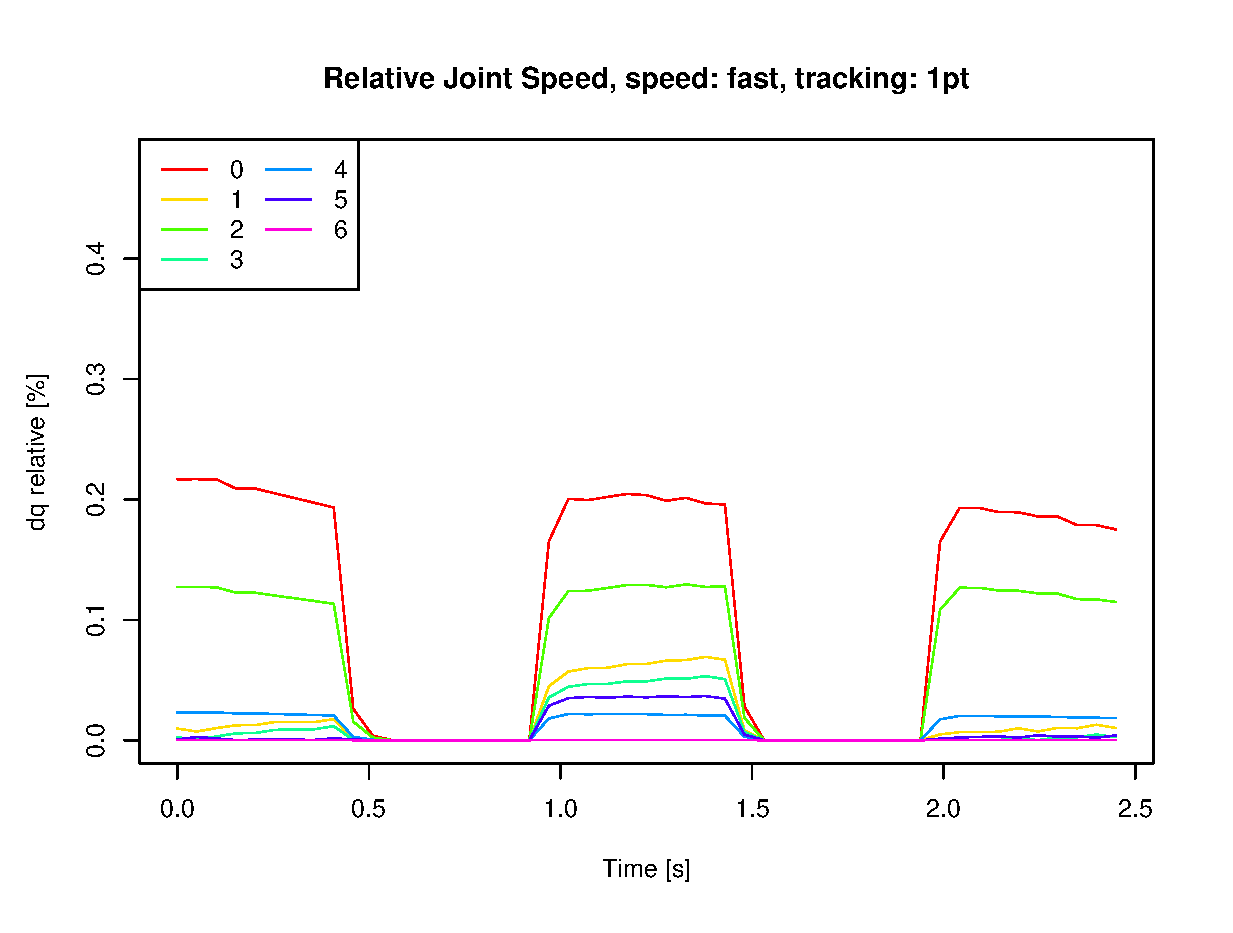
\includegraphics[width= \linewidth]{graphics/robotics/relativeConfVel_fast_1pt}
\caption{Robot speed relative to the velocity limit. 
Tracking one point using fast marker movement.}
\label{fig:robotspeed_fast_1p}
\end{figure}

% ---------- tool pose ----------
\begin{figure}[H]
\centering
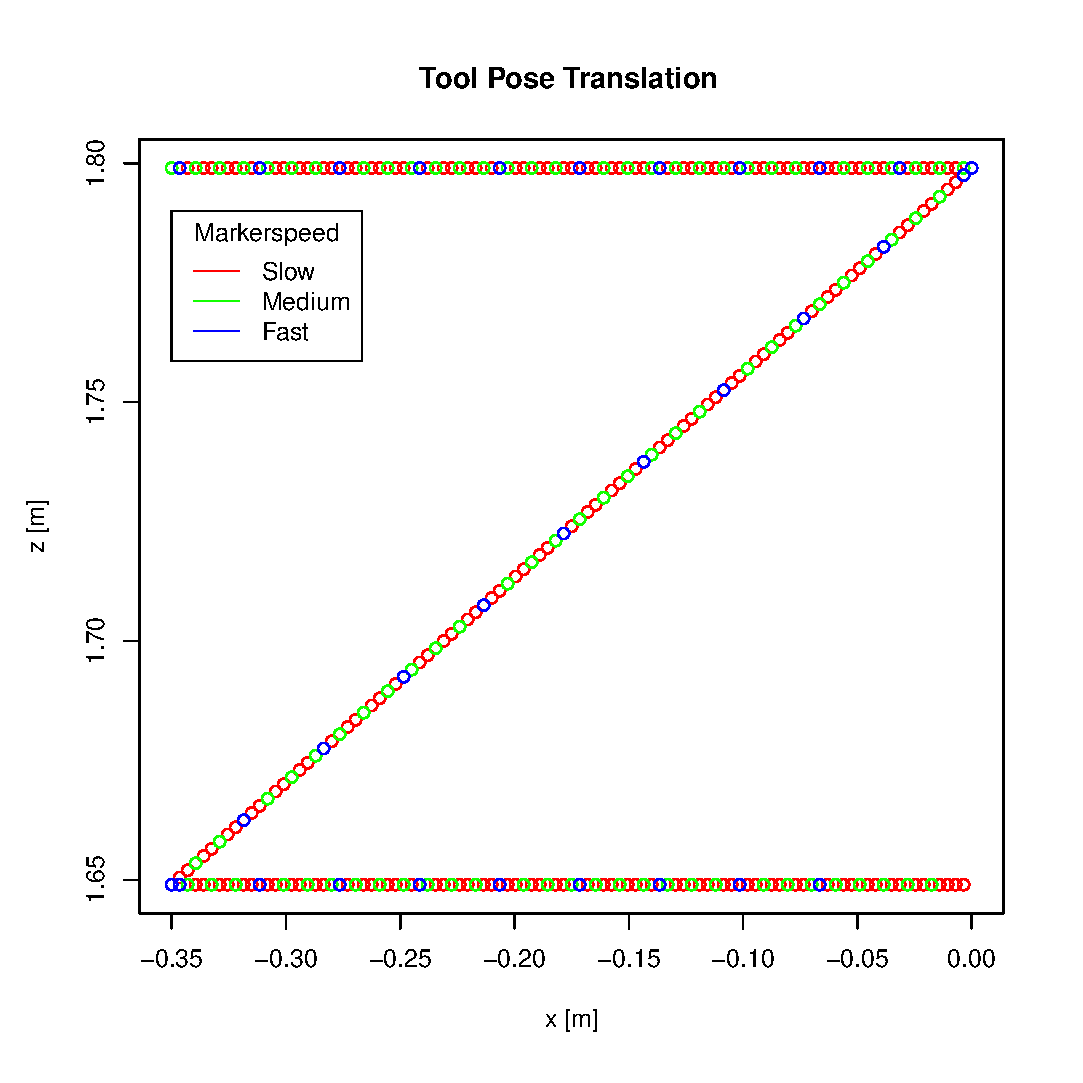
\includegraphics[width= \linewidth]{graphics/robotics/toolPose_1pt_pos}
\caption{Translational part of tool pose when tracking the marker placement in the image.}
\label{fig:toolpose_1p_pos}
\end{figure}

\begin{figure}[H]
\centering
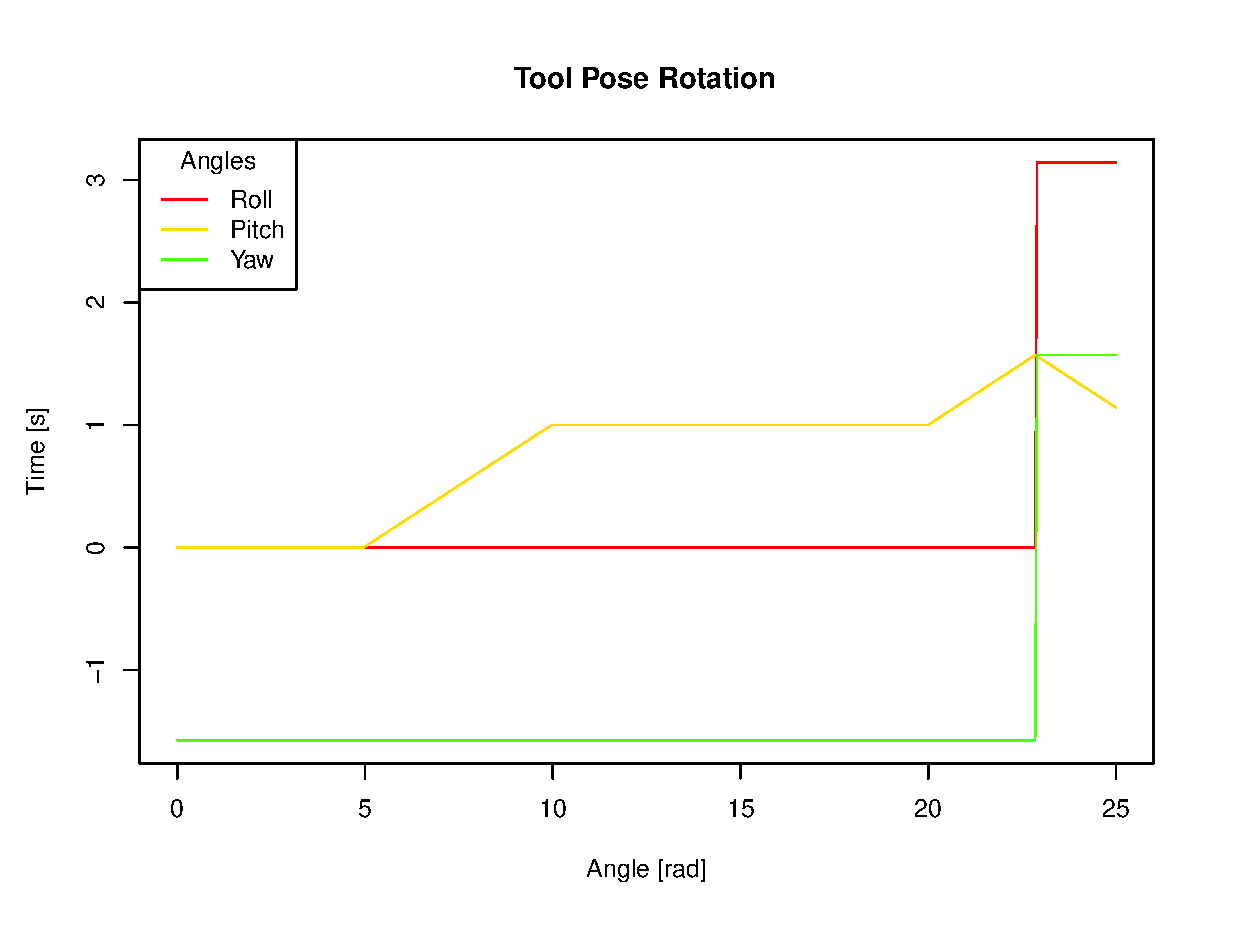
\includegraphics[width= \linewidth]{graphics/robotics/toolPose_slow_1pt}
\caption{RPY part of tool pose. Using the slow marker movement while tracking 1 point.}
\label{fig:toolpose_slow_1p_rpy}
\end{figure}

\begin{figure}[H]
\centering
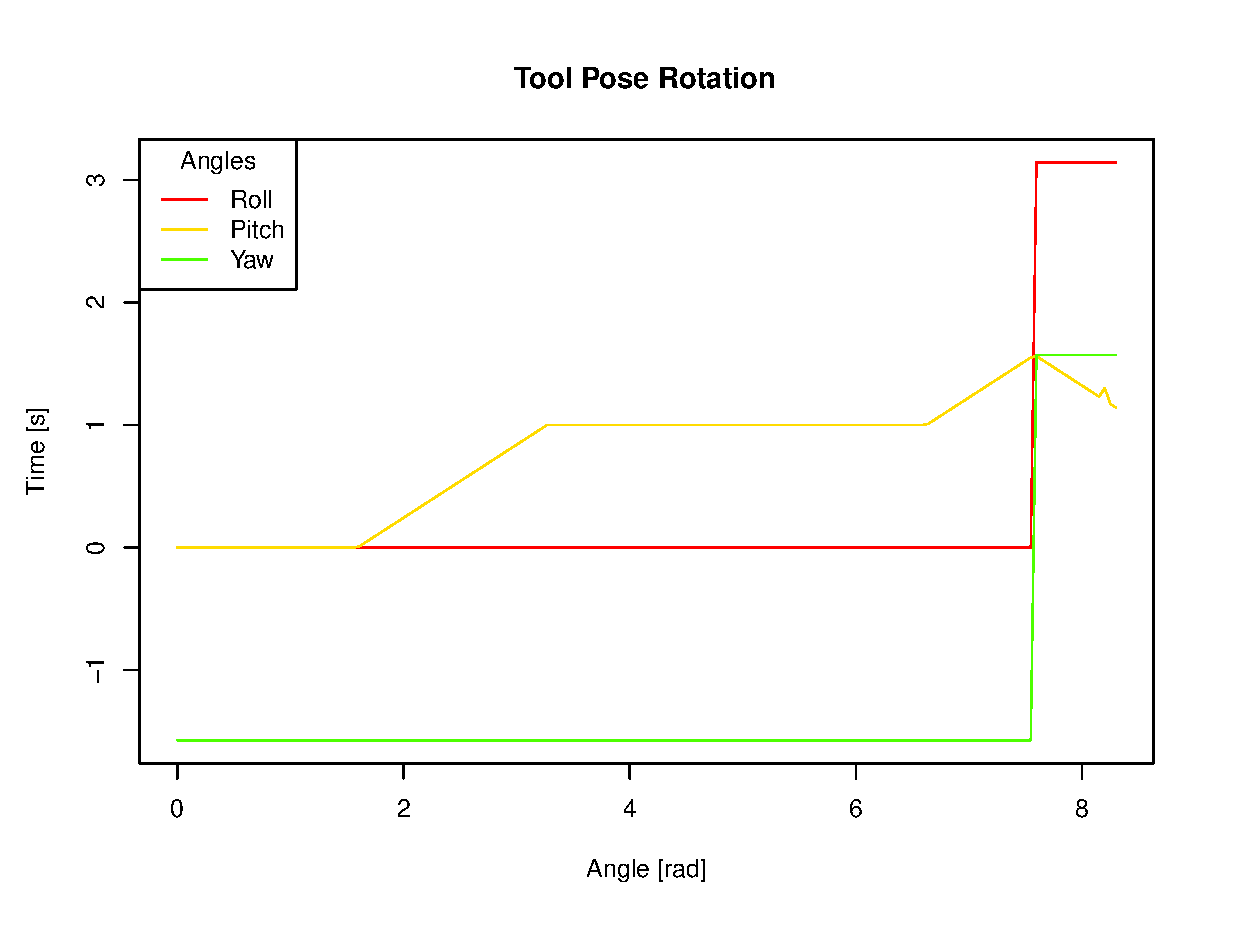
\includegraphics[width= \linewidth]{graphics/robotics/toolPose_medium_1pt}
\caption{RPY part of tool. Using the medium marker movement while tracking 1 point.}
\label{fig:toolpose_medium_1p_rpy}
\end{figure}

\begin{figure}[H]
\centering
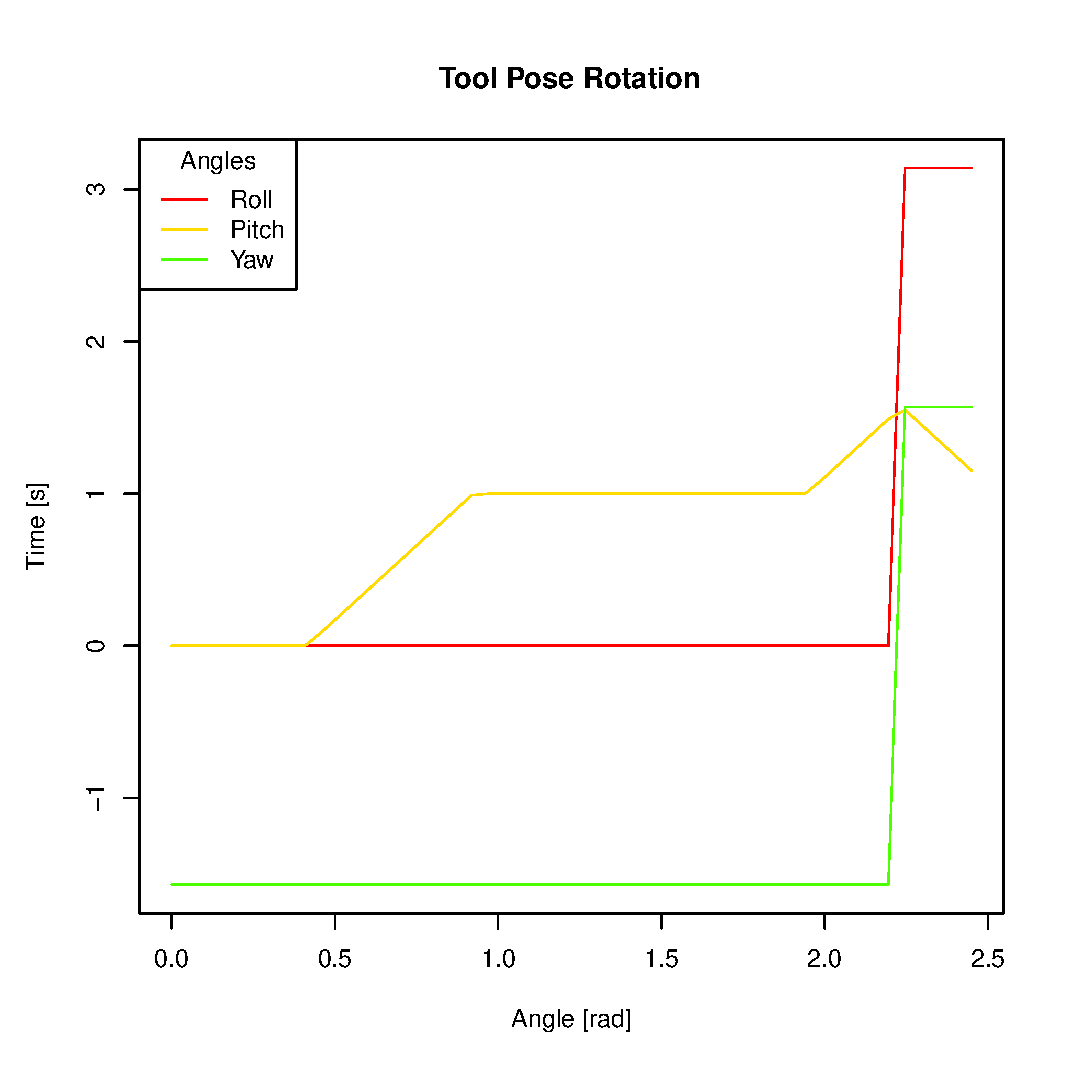
\includegraphics[width= \linewidth]{graphics/robotics/toolPose_fast_1pt}
\caption{RPY part of tool pose. Using the fast marker movement while tracking 1 point.}
\label{fig:toolpose_fast_1p_rpy}
\end{figure}


% ---------- tracking error ----------
\begin{figure}[H]
\centering
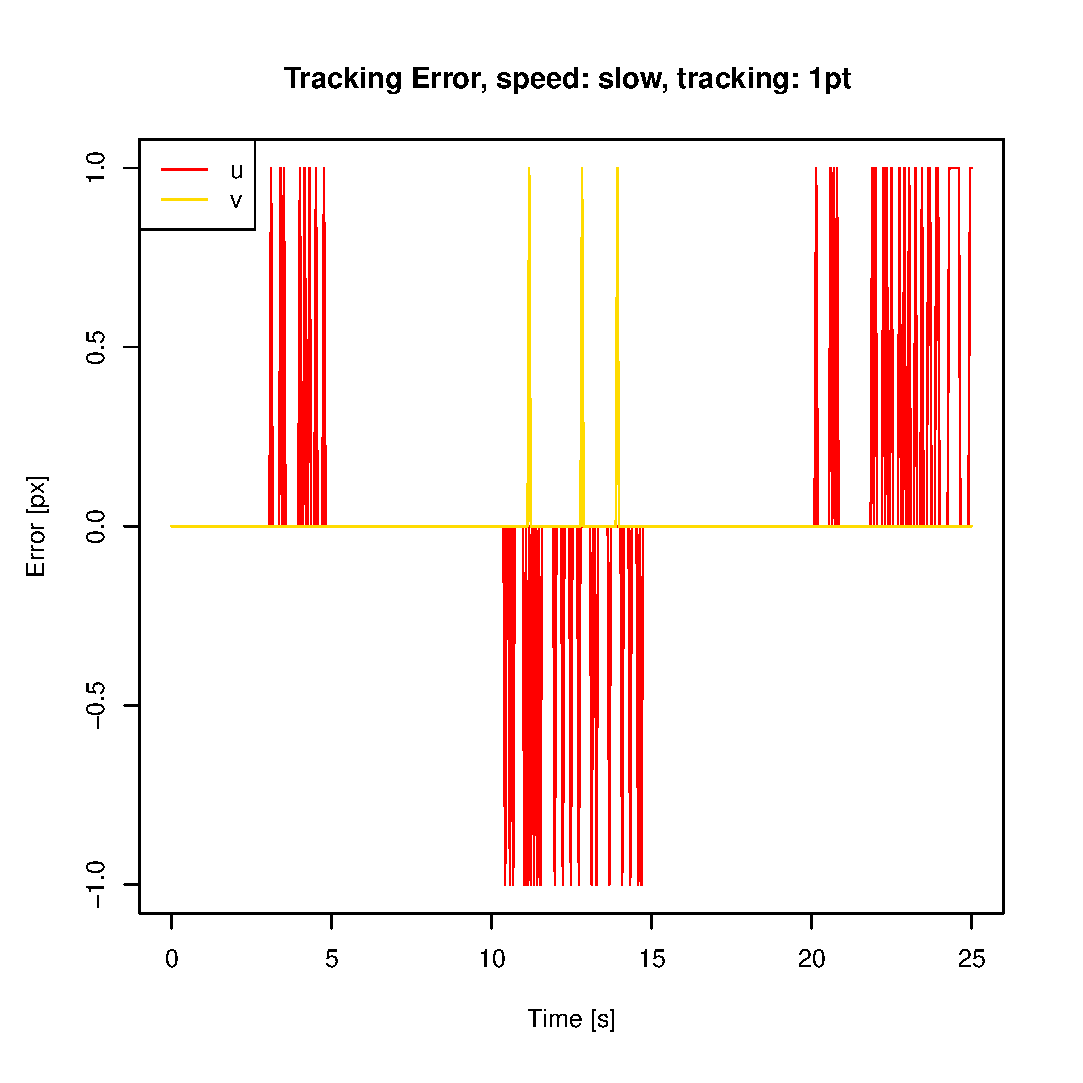
\includegraphics[width= \linewidth]{graphics/robotics/trackingError_slow_1pt}
\caption{Tracking error in image coordinates.
Following the marker for the slow marker movement.}
\label{fig:trackingerror_slow_1p}
\end{figure}

\begin{figure}[H]
\centering
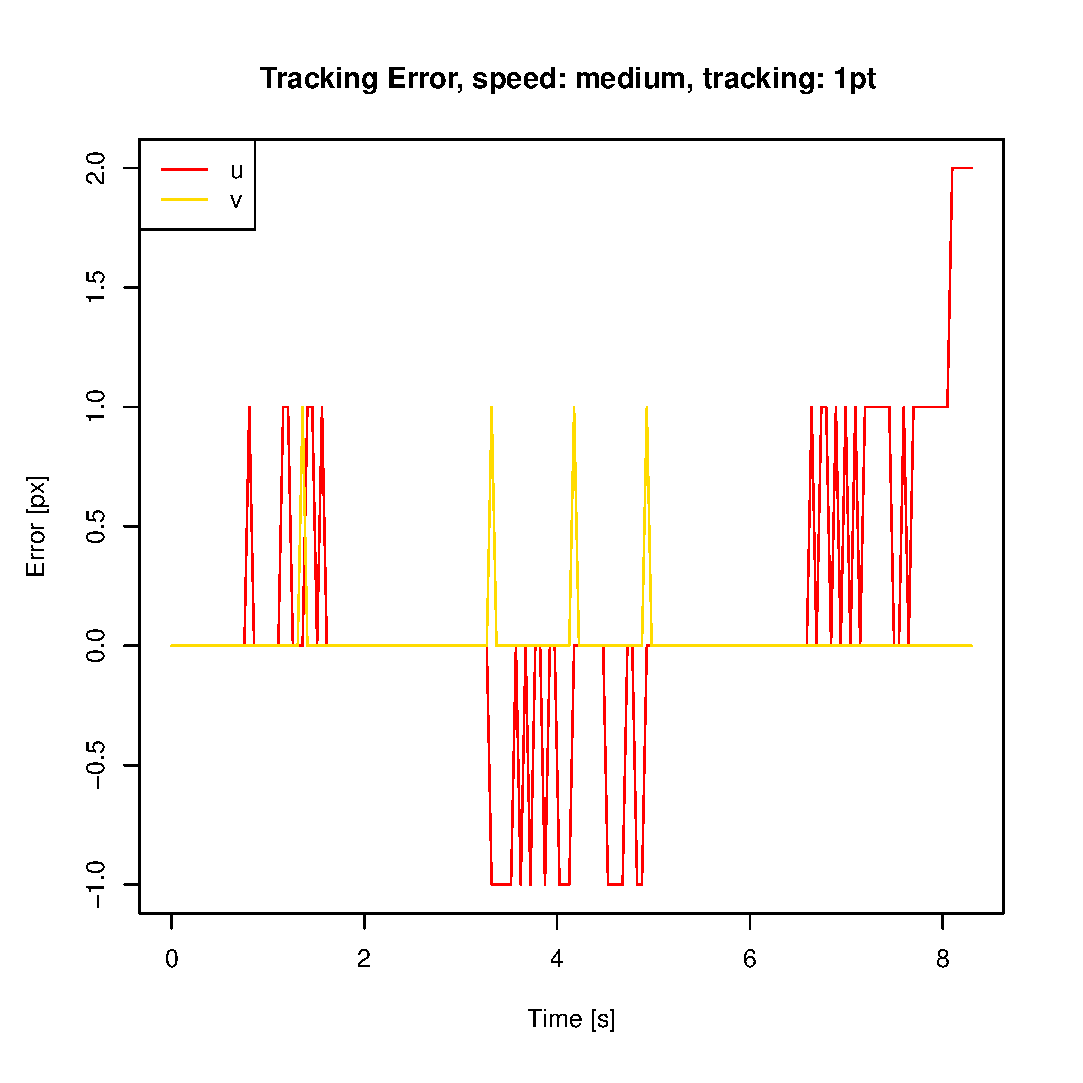
\includegraphics[width= \linewidth]{graphics/robotics/trackingError_medium_1pt}
\caption{Tracking error in image coordinates.
Following the marker for the medium marker movement.}
\label{fig:trackingerror_medium_1p}
\end{figure}


\begin{figure}[H]
\centering
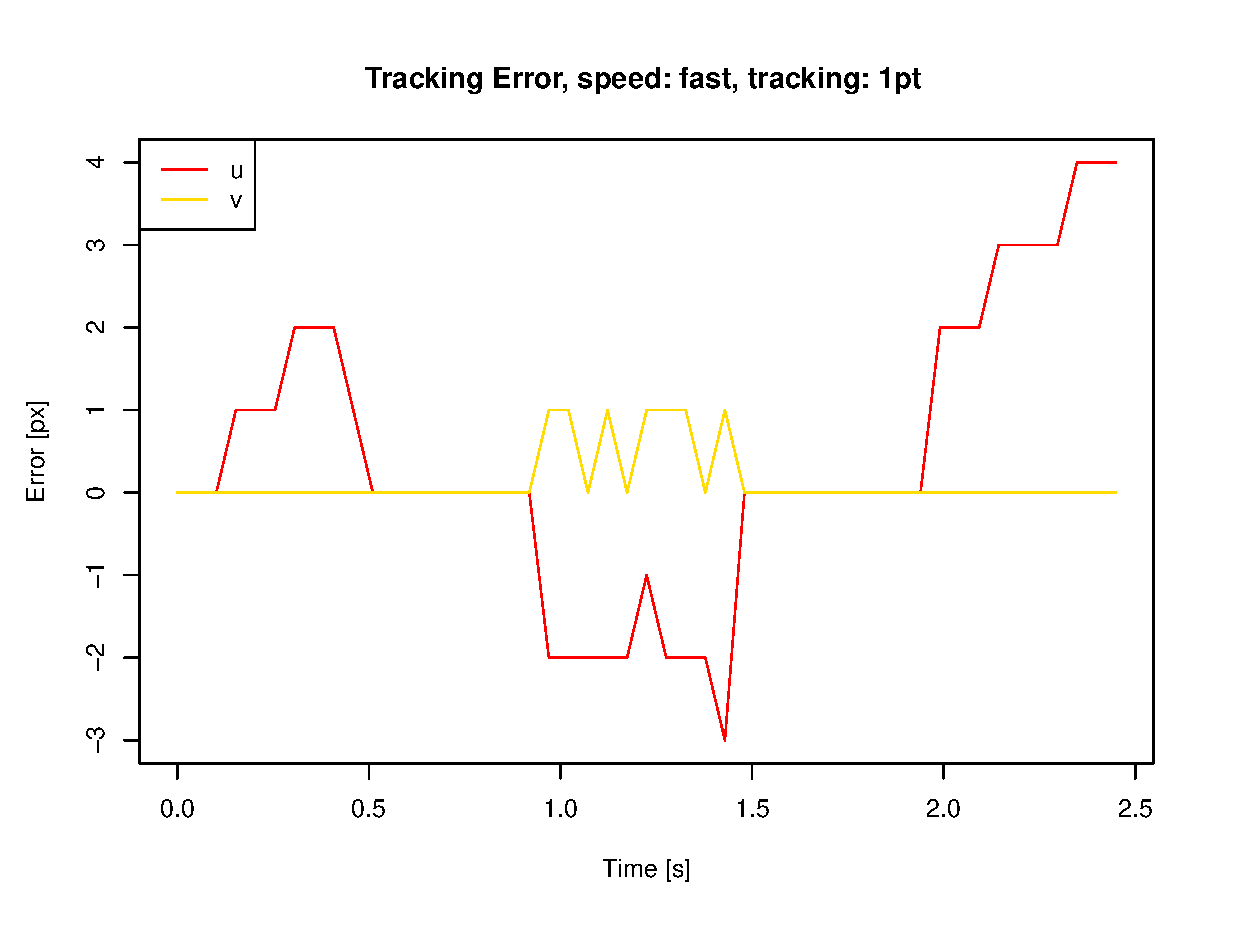
\includegraphics[width= \linewidth]{graphics/robotics/trackingError_fast_1pt}
\caption{Tracking error in image coordinates.
Following the marker for the fast marker movement.}
\label{fig:trackingerror_fast_1p}
\end{figure}


%Since these numbers should be the closest to ground truth achievable, then these will also be used in comparisons in section \ref{sec:combinedSystem} when the whole system is brought together in the simulation.

It was found that in none of the cases was the velocity constraint violated for all of the datasets down to a $\Delta t = 0.05$ seconds in between each frame.
The tracking error does also increase as the marker movement speed increases, but the path taken by the robot tool is more or less the same for all of the datasets.


